%% LyX 2.1.4 created this file.  For more info, see http://www.lyx.org/.
%% Do not edit unless you really know what you are doing.
\RequirePackage{fixltx2e}
\documentclass[english,t]{beamer}
\usepackage[T1]{fontenc}
\usepackage[latin9]{inputenc}
\setcounter{secnumdepth}{3}
\setcounter{tocdepth}{3}
\synctex=-1
\usepackage{booktabs}
\usepackage{fancybox}
\usepackage{calc}
\usepackage{amsmath}
\usepackage{cancel}
\usepackage{graphicx}
\usepackage{esint}

\makeatletter

%%%%%%%%%%%%%%%%%%%%%%%%%%%%%% LyX specific LaTeX commands.
\newcommand{\noun}[1]{\textsc{#1}}
%% Because html converters don't know tabularnewline
\providecommand{\tabularnewline}{\\}

%%%%%%%%%%%%%%%%%%%%%%%%%%%%%% Textclass specific LaTeX commands.
 % this default might be overridden by plain title style
 \newcommand\makebeamertitle{\frame{\maketitle}}%
 % (ERT) argument for the TOC
 \AtBeginDocument{%
   \let\origtableofcontents=\tableofcontents
   \def\tableofcontents{\@ifnextchar[{\origtableofcontents}{\gobbletableofcontents}}
   \def\gobbletableofcontents#1{\origtableofcontents}
 }

\@ifundefined{date}{}{\date{}}
%%%%%%%%%%%%%%%%%%%%%%%%%%%%%% User specified LaTeX commands.
\usetheme{rwth}
\usepackage{braket}

\title{Polarimetry for Storage Ring EDM experiments}
\subtitle{\vspace{2cm} \hspace{15cm} \includegraphics{jedi_logo2.png} \vspace{-2cm}}
\author{Paul Maanen}
\institute{Physics Institute III B, RWTH Aachen University}
\date[July 1, 2016]{Friday Seminar July 1, 2016}

% Some changes on the layout, can be switched off by commenting out
\setheadlinestyle{headlineframetitle}
\setfooterstyle{footertitleauthor}
\setfootlinestyle{footlinedatepages}

% German style date formatting (footer)
\usepackage[ddmmyyyy]{datetime}
\renewcommand{\dateseparator}{.}

% To get greek letters better matching with rest of font
\usepackage{upgreek}

\logo{\includegraphics{rwth_3physik_b_englisch_rgb.png}}

\newif\ifexperimentlogo %-> defines a boolean variable for an if-case
\experimentlogotrue     %-> sets it true(\experimentlogotrue)/false(\experimentlogofalse); !: no spaces between
% \pgfdeclareimage[options]{name}[file}
\pgfdeclareimage[height=13mm,interpolate=true]{experimentLogo}{jedi_logo2.png} %links a logo to the name experimentlogo 
\AtBeginSection[]{
  \begin{frame}[plain, noframenumbering]{}
  \vfill
  \centering
  \begin{beamercolorbox}[sep=8pt,center,shadow=true,rounded=true]{title}
    \usebeamerfont{title}\insertsectionhead\par%
  \end{beamercolorbox}
  \vfill
  \end{frame}
}

\makeatother

\usepackage{babel}
\begin{document}
\setbeamercolor{title page bar}{fg=rwth} 
\setbeamertemplate{title page}[rwth]{} 
\begin{frame}[plain, noframenumbering]{}


\titlepage
\end{frame}

\begin{frame}[plain, noframenumbering]{Outline}


\tableofcontents{}

\end{frame}



\section{Motivation}
\begin{frame}{Motivation}

\begin{description}
\item [{Where}] is the Antimatter in our Universe? 
\end{description}

\vspace{5mm}

\begin{itemize}
\item Sakharov (1967): Three conditions for baryogenesis

\begin{itemize}
\item At least one Baryon-number violating process.
\item $\cancel{\mathcal{C}}$and $\cancel{\mathcal{CP}}$
\item Interactions outside of thermal equilibrium. 
\end{itemize}
\end{itemize}

\vspace{5mm}

\begin{itemize}
\item Baryon number asymmetry: $\frac{n_{B}-n_{\overline{B}}}{n_{\gamma}}\approx\begin{cases}
10^{-18} & (SM)\\
10^{-10} & (Exp.)
\end{cases}$
\end{itemize}

\vspace{5mm}

\begin{description}
\item [{$\Rightarrow$Not}] enough $\cancel{\mathcal{CP}}$ in Standard
Modell
\end{description}
\end{frame}

\begin{frame}{Electric Dipole Moments}

\begin{itemize}
\item Classical Electric Dipole Moment: Charge separation
\item Interaction of electric and magnetic dipole moments with $\vec{E},\vec{B}$:
\end{itemize}

\begin{center}
\begin{tabular}{l}
\phantom{$\mathcal{P}$: }$\mathcal{H}=-\mu\frac{\vec{S}}{S}\cdot\vec{B}\textcolor{red}{\ensuremath{-}}d\frac{\vec{S}}{S}\cdot\vec{E}$\tabularnewline
$\mathcal{P}$: $\mathcal{H}=-\mu\frac{\vec{S}}{S}\cdot\vec{B}\textcolor{red}{\ensuremath{+}}d\frac{\vec{S}}{S}\cdot\vec{E}$\tabularnewline
$\mathcal{T}$: $\mathcal{H}=-\mu\frac{\vec{S}}{S}\cdot\vec{B}\textcolor{red}{\ensuremath{+}}d\frac{\vec{S}}{S}\cdot\vec{E}$\tabularnewline
\end{tabular}\hspace{1cm}%
\Ovalbox{\parbox[c][1\totalheight][t]{0.25\textwidth}{%
\begin{center}
$\vec{d}=EDM$\\
$\vec{\mu}=MDM$\\
$\vec{\mu},\vec{d}\parallel\vec{S}$\\
$\cancel{T}\overset{\mathcal{CPT}}{\Leftrightarrow}\cancel{\mathcal{CP}}$
\par\end{center}%
}}
\par\end{center}
\begin{description}
\item [{$\Rightarrow$Electric\ Dipole\ Moments}] violate $\mathcal{CP}$
(assuming $\mathcal{CPT}$)
\item [{$\Rightarrow$Probe}] into the Physics of the early universe
\end{description}
\end{frame}

\begin{frame}{Charged particle EDMs: Current Limits and Challenges }

\begin{itemize}
\item Most EDM searches measure EDM of neutral particles. Current Limits
$10^{-17}e\mathrm{cm}-10^{-28}e\mathrm{cm}$
\end{itemize}

\vspace{5mm}

\begin{itemize}
\item No direct limits for charged hadrons exist

\begin{itemize}
\item Technical challenge: No trap for charged particles

\begin{description}
\item [{$\Rightarrow$Storage~Ring~needed!}]~
\end{description}
\end{itemize}
\end{itemize}

\vspace{5mm}

\begin{itemize}
\item EDM search @ FZJ: $\mathrm{p},\mbox{\ensuremath{\mathrm{\textcolor{red}{d}}}},\mathrm{^{3}He}$
\end{itemize}

\vspace{-20mm}



\begin{flushright}
\includegraphics[height=8cm]{gfx/edm_current_limits_goals}
\par\end{flushright}

\end{frame}

\begin{frame}{EDM searches in storage rings}

\begin{itemize}
\item All EDM experiments measure interaction between $\vec{d}$ and $\vec{E}$:

\begin{itemize}
\item $\frac{d\vec{S}}{dt}\propto d\vec{E}\times\vec{S}$
\end{itemize}

\vspace{5mm}


\item ``Frozen Spin'' method: Align spin with momentum vector, wait for
vertical polarization change: 

\begin{itemize}
\item $\frac{\Delta S_{y}}{\Delta t}\propto d$
\end{itemize}
\end{itemize}

\vspace{5mm}



\begin{flushright}
\includegraphics[height=7.5cm]{gfx/idea}
\par\end{flushright}


\vspace{-95mm}

\begin{itemize}
\item Current candidate method for EDM search implicates a buildup of polarization
with time at $\Delta P=\mathcal{O}(10^{-6}/1000s)$
\end{itemize}
\end{frame}

\begin{frame}{Nuclear scattering polarimetry}

\begin{itemize}
\item Nuclear scattering cross section for scattering of polarized particles:
$\sigma_{L,R}=\sigma_{0}\cdot\big(1\pm P_{y}A_{y}\big)$\vspace{5mm}

\item Measure left-right asymmetries in count rate: $P_{y}=\frac{1}{A_{y}}\frac{N_{L}-N_{R}}{N_{L}+N_{R}}$\vspace{5mm}

\item Up and Down counting rates may be used to control systematics\vspace{5mm}

\end{itemize}

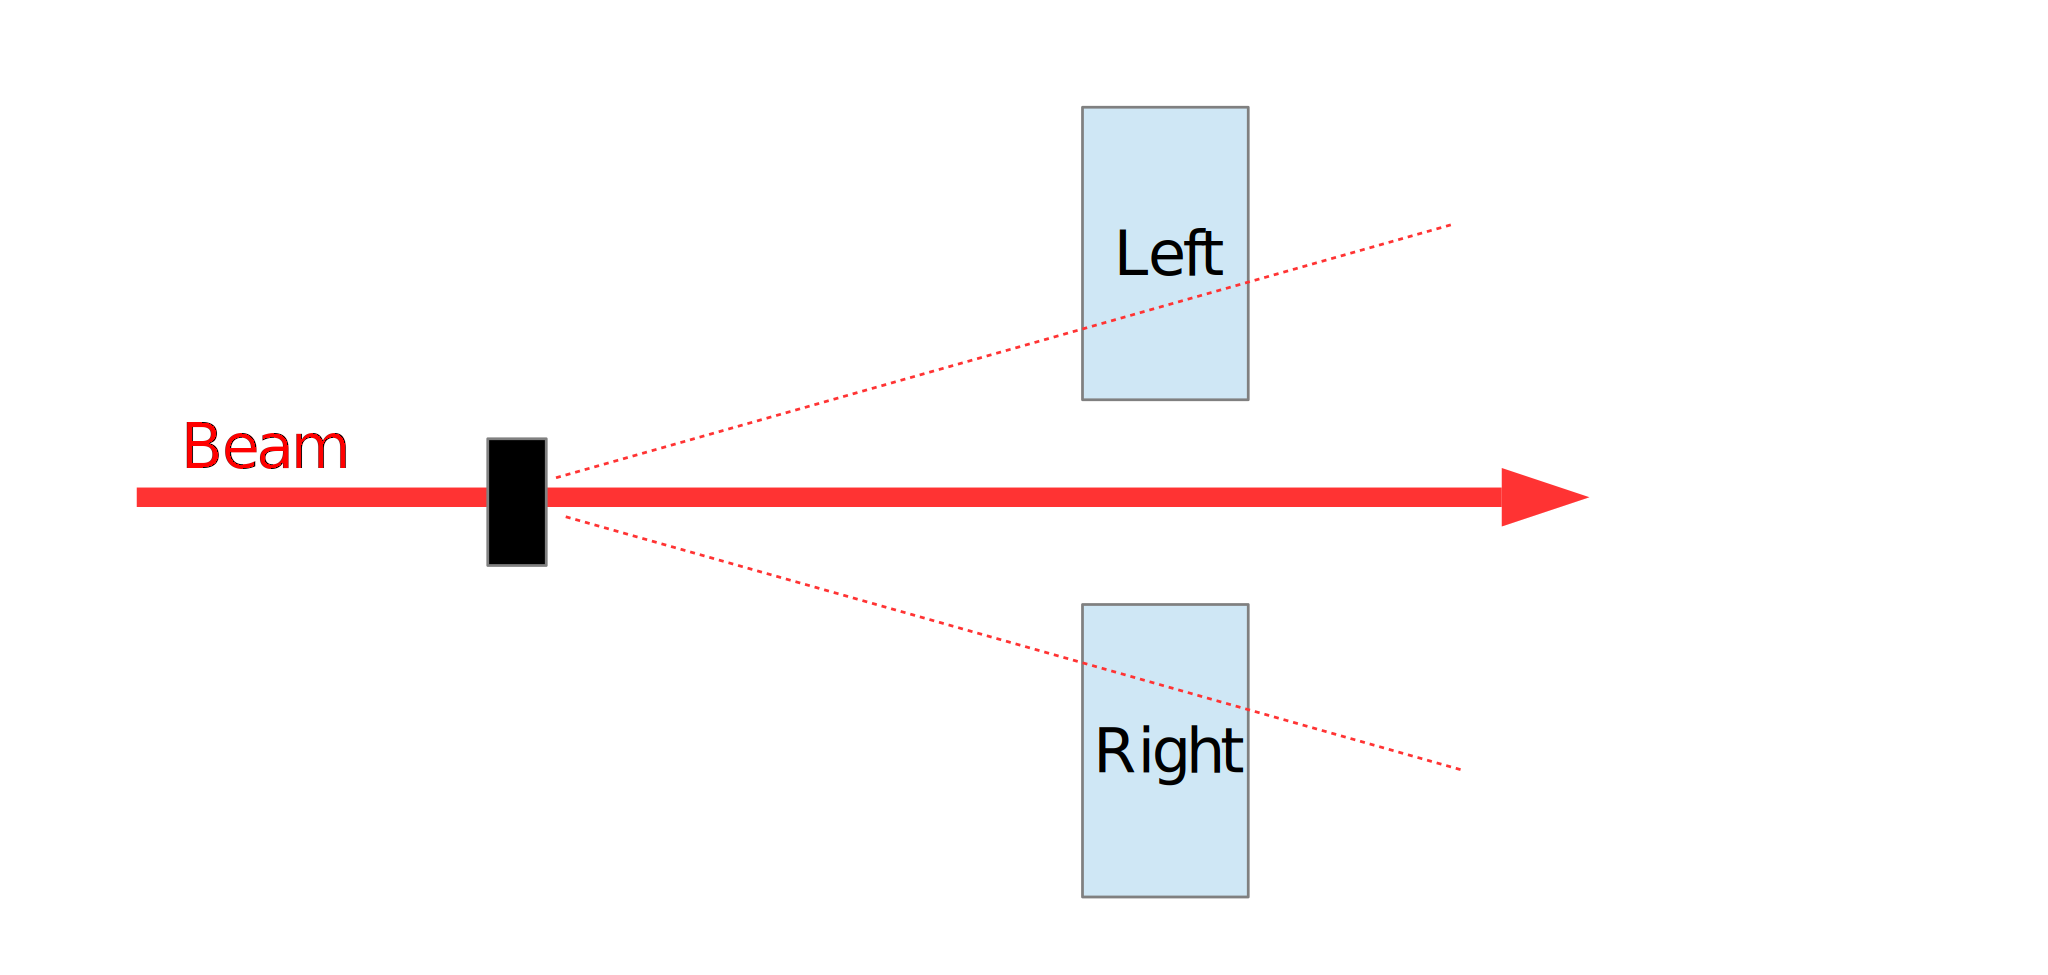
\includegraphics[height=0.5\textheight]{gfx/left-right}

\end{frame}

\begin{frame}{Design goals for an EDM polarimeter}

\begin{itemize}
\item Design goals for polarimeter:

\begin{itemize}
\item Large statistical Figure-of-Merit: $\mathcal{FOM\sim}N\cdot(P_{y}A_{y})^{2}$\vspace{5mm}

\item Minimal influence on beam\vspace{5mm}

\item Good handle on systematic effects\vspace{5mm}

\item Good long term stability and reproducibility: $1$ppm per $1000s$
\end{itemize}
\end{itemize}

\end{frame}



\section{Polarimeter concept}
\begin{frame}{Reaction choice}




\begin{center}
\includegraphics[height=0.6\textheight]{gfx/FOM}
\par\end{center}
\begin{itemize}
\item Carbon is the current material of choice
\item $\mathcal{FOM}$ concentrated in forward region

\begin{description}
\item [{$\Rightarrow$Polarimeter~needs~to~cover~forward~region}]~
\end{description}
\item Proton-Carbon elastic scattering also concentrated in forward region.

\begin{description}
\item [{$\Rightarrow$Possibility}] for multi-purpose polarimeter
\end{description}
\end{itemize}
\end{frame}

\begin{frame}{Detector concept}


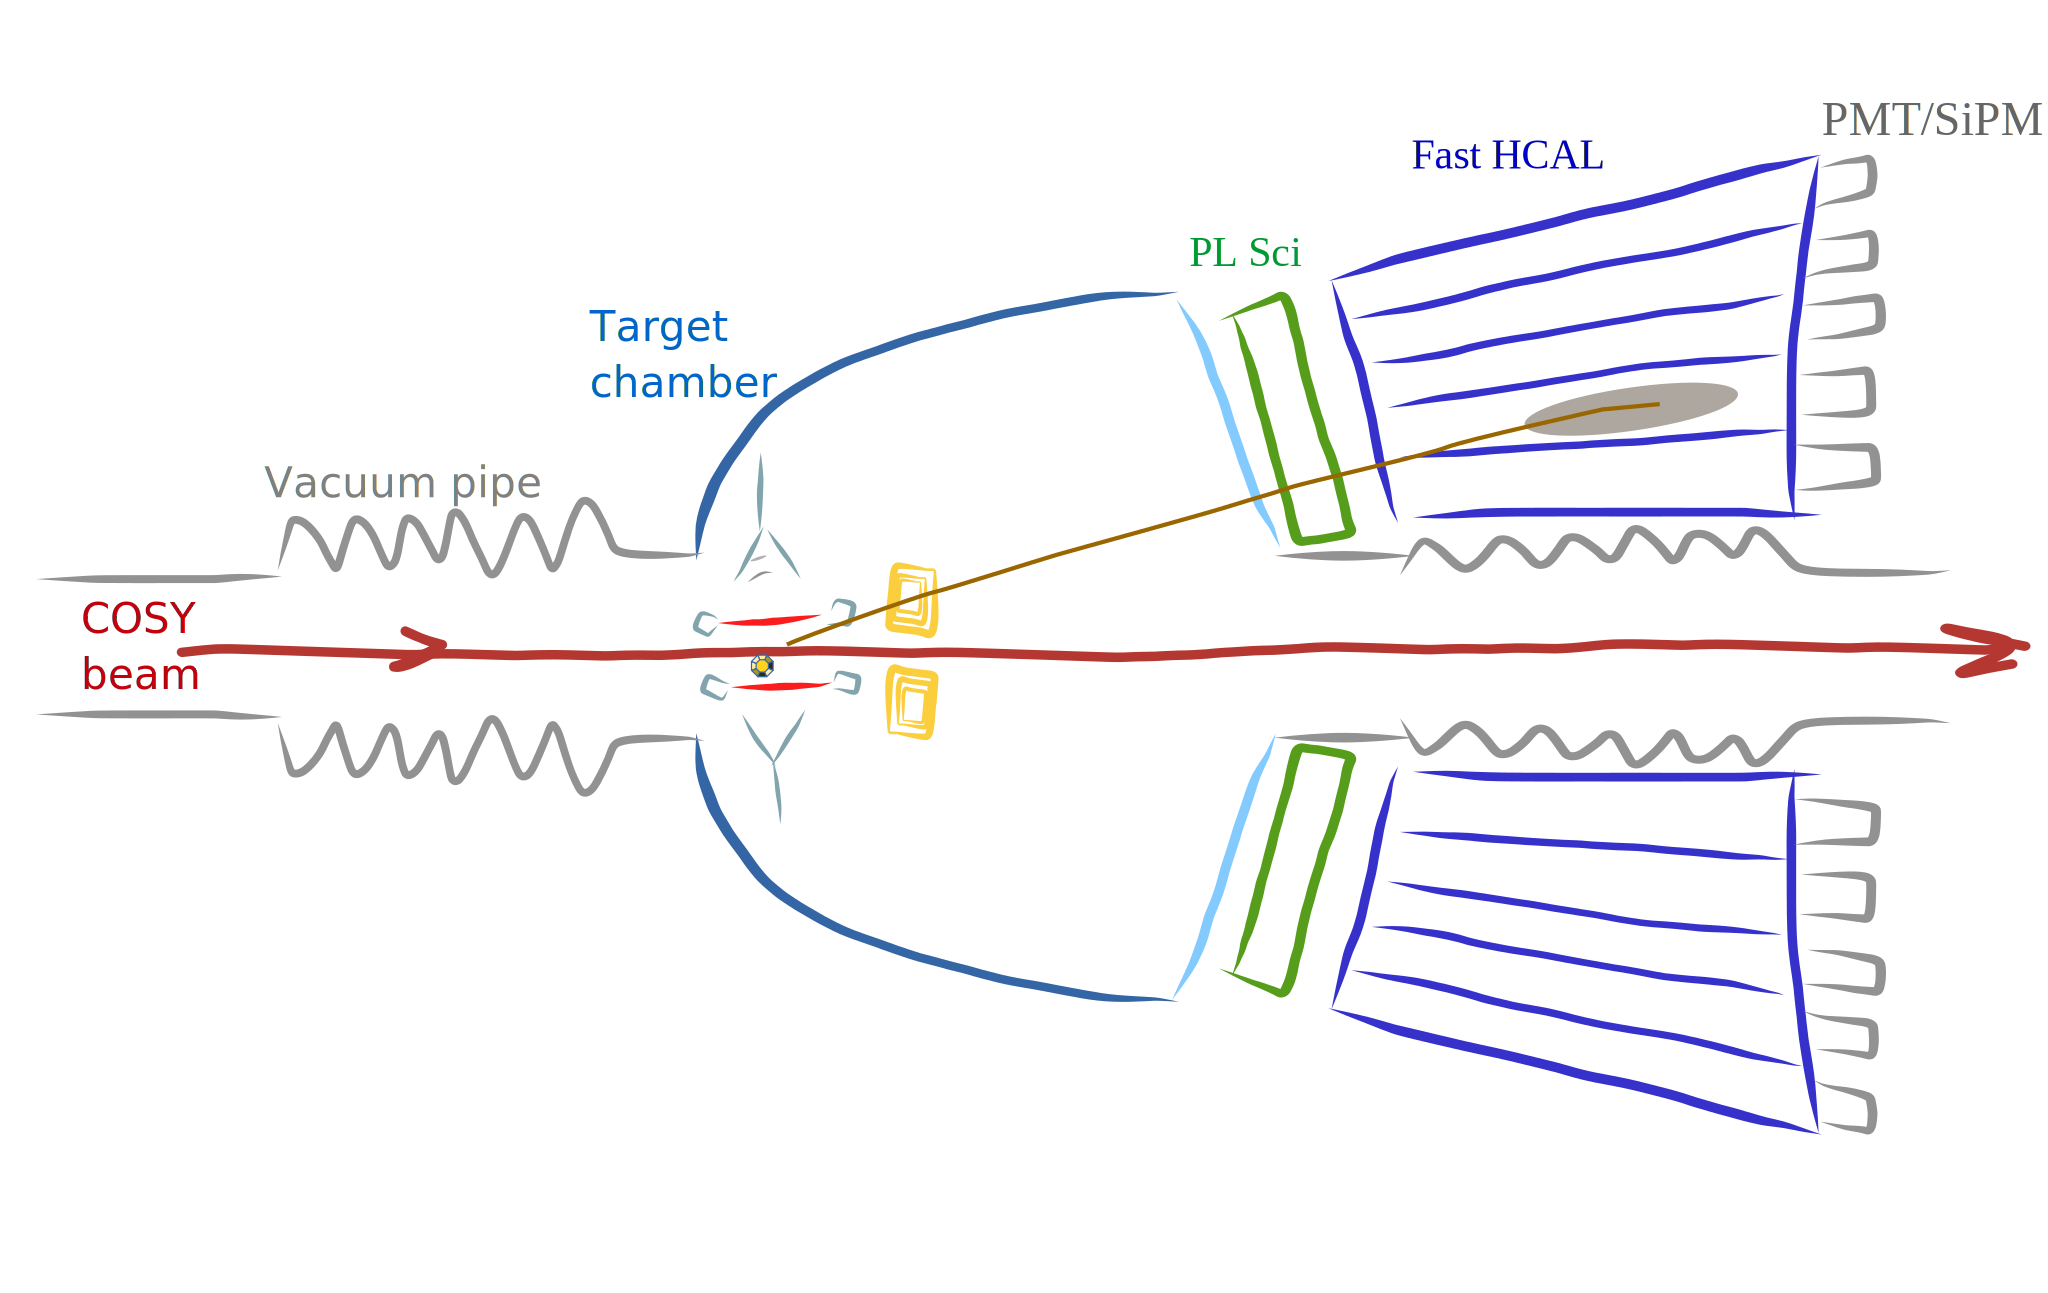
\includegraphics[height=1\textheight]{gfx/DetectorSketch}

\end{frame}

\begin{frame}{Target concept}


\includegraphics[height=1\textheight]{gfx/target}

\end{frame}

\begin{frame}{Readout concept}


\includegraphics[height=1\textheight]{gfx/readout}

\end{frame}



\section{Simulation studies}
\begin{frame}{HCal Candidate Materials: LYSO/Plastic Scintillator }


\begin{center}
\begin{tabular}{c}
\includegraphics[width=0.3\textwidth]{gfx/lyso-sketch}\tabularnewline
\vspace{1cm}
\tabularnewline
\includegraphics[width=0.3\textwidth]{gfx/plastic-sketch}\tabularnewline
\end{tabular}\hspace{1cm}%
\begin{tabular}{ccc}
\toprule 
 & LYSO & Plastic\tabularnewline
\midrule
\midrule 
Stopping power & + & -\tabularnewline
\midrule
\midrule 
Speed & + & +\tabularnewline
\midrule
\midrule 
Energy resolution & + & -\tabularnewline
\midrule
\midrule 
Cost & - & +\tabularnewline
\bottomrule
\end{tabular}
\par\end{center}

\end{frame}

\begin{frame}{First step: Detector element dimensions}


\includegraphics[width=0.45\textwidth]{gfx/simulation-single}\hspace{0.05\textwidth}\includegraphics[width=0.45\textwidth]{gfx/simulation-sandwich}


\vspace{5mm}

\begin{itemize}
\item Open Questions:

\begin{itemize}
\item Optimal calorimeter element size?
\item Absorber Thickness?
\item Monolithic or Sandwich?
\item Plastic or LYSO?
\end{itemize}
\end{itemize}
\end{frame}

\begin{frame}{Detector dimensions - LYSO\includegraphics[height=0.1\textheight]{gfx/lyso-sketch}}


\begin{flushright}

\par\end{flushright}


\includegraphics[width=0.5\textwidth]{gfx/lyso-range}\includegraphics[width=0.5\textwidth]{gfx/lyso-x}


\vspace{5mm}

\begin{itemize}
\item To get lateral and longitudinal range of deuteron in detector element:

\begin{itemize}
\item Shoot particle gun into front face, determine $x_{f},y_{f},z_{f}$
of endpoint of primary track
\item Longitudinal range: Gaussian fit
\item Lateral width: $\int_{-x0}^{x0}dN/dx=90\%\cdot N_{tot}$
\end{itemize}

\vspace{5mm}


\item Chosen detector size of $3\times3\times10\,$$\mathrm{cm}^{3}$ as
starting point for further studies
\end{itemize}
\end{frame}

\begin{frame}{Detector response - LYSO\includegraphics[height=0.1\textheight]{gfx/lyso-sketch}}


\includegraphics[width=0.8\textwidth]{gfx/cocktail-lyso}
\begin{itemize}
\item Breakup in detector element causes distortion of energy spectrum
\end{itemize}
\end{frame}

\begin{frame}{Detector dimensions - Plastic\includegraphics[height=0.1\textheight]{gfx/plastic-sketch}}


\includegraphics[width=0.5\textwidth]{gfx/thickness}\includegraphics[width=0.45\textwidth]{../DPG2016/deuteron-plastic-100-range}


\vspace{5mm}

\begin{itemize}
\item Use absorber to suppress proton background and reduce length of plastic
detector
\end{itemize}

\vspace{5mm}

\begin{itemize}
\item Arbitrarily chosen $100\,\mathrm{MeV}$ entry energy @ $270\,\mbox{MeV}$
beam energy as working point for plastic scintillator

\begin{itemize}
\item Iron thickness ca. $50\,\mbox{mm}$ 
\item Pl. scintillator thickness ca. $50\,\mbox{mm}$
\end{itemize}



\end{itemize}
\end{frame}

\begin{frame}{Detector response - Plastic\includegraphics[height=0.1\textheight]{gfx/plastic-sketch}}


\includegraphics[width=0.8\textwidth]{gfx/cocktail-plastic}

\end{frame}

\begin{frame}{Next step(s): Monolithic or sandwich detector? }


\includegraphics[width=0.45\textwidth]{gfx/simulation-single}\hspace{0.05\textwidth}\includegraphics[width=0.45\textwidth]{gfx/simulation-sandwich}
\begin{itemize}
\item Generated 100k events each at $T_{d}=270\,\mathrm{MeV}$,$5^{\circ}<\Theta<20^{\circ}$,
$0^{\circ}<\phi<360^{\circ}$

\begin{itemize}
\item Signal: $^{12}C(\vec{d},d)^{12}C$,$\sigma_{el}\approx X\mbox{\,mb}$
,$<A_{y}>\approx$
\item Background: $^{12}C(\vec{d},pn)^{12}C$,$\sigma_{el}\approx X\mbox{\,mb}$
,$<A_{y}>\approx$
\end{itemize}
\end{itemize}

\vspace{5mm}

\begin{itemize}
\item $\mathcal{FOM}\propto\sigma_{eff}\times<A_{y,eff}>^{2}$
\end{itemize}
\end{frame}

\begin{frame}{Signal and Background generation}




\includegraphics[width=0.5\textwidth]{gfx/hDeuteron}\includegraphics[width=0.5\textwidth]{gfx/hCarbon}


\vspace{5mm}

\begin{itemize}
\item Using data-driven model for signal and background
\end{itemize}

\vspace{5mm}

\begin{itemize}
\item Elastically scattered deuterons retain almost complete beam energy
\end{itemize}

\vspace{5mm}

\begin{itemize}
\item Contribution of recoil carbons negligible
\end{itemize}
\end{frame}

\begin{frame}{Signal and Background generation (cont'd)}


\includegraphics[width=0.5\textwidth]{gfx/hProton}\includegraphics[width=0.5\textwidth]{gfx/hNeutron}
\begin{itemize}
\item Break-up has almost no analyzing power, so discard it
\end{itemize}

\vspace{5mm}

\begin{itemize}
\item Protons and neutrons from break-up are energetically well separated
from signal

\begin{description}
\item [{$\Rightarrow$But:}] Break-up in target is not distinguishable
from break-up in detector!
\end{description}

\vspace{5mm}


\item No reliable model for inelastic reactions available

\begin{itemize}
\item Qualitative experiments show: Inelastic reactions carry some analysing
power, so maybe keep these
\end{itemize}
\end{itemize}
\end{frame}

\begin{frame}{Detection efficiencies (lyso)\includegraphics[height=0.1\textheight]{gfx/lyso-sketch}}


\includegraphics[width=0.45\textwidth]{gfx/lyso-dcelastic}\includegraphics[width=0.45\textwidth]{gfx/lyso-dcbreakup}


\includegraphics[width=0.45\textwidth]{gfx/fom-lyso}

\end{frame}

\begin{frame}{Detection efficiencies (plastic)\includegraphics[height=0.1\textheight]{gfx/plastic-sketch}}




\includegraphics[width=0.45\textwidth]{gfx/plastic-dcelastic}\includegraphics[width=0.45\textwidth]{gfx/plastic-dcbreakup}


\includegraphics[width=0.45\textwidth]{gfx/fom-plastic}

\end{frame}

\begin{frame}{Simulation Results}

\begin{itemize}
\item Main cause of efficiency loss is breakup in detector
\end{itemize}

\vspace{5mm}

\begin{itemize}
\item Maximum relative FOM:
\end{itemize}

\vspace{2mm}



\hspace{2cm}%
\begin{tabular}{ccc}
\toprule 
 & 0\% & 20\%\tabularnewline
\midrule
\midrule 
Plastic & 15.5 & 14.5\tabularnewline
\midrule
\midrule 
LYSO & 17 & 12\tabularnewline
\bottomrule
\end{tabular}


\vspace{5mm}

\begin{itemize}
\item LYSO and plastic scintillators provide comparable performance
\end{itemize}

\vspace{5mm}

\begin{itemize}
\item Plastic scintillator performance exhibits no strong dependence on
energy resolution 
\end{itemize}
\end{frame}

\section{R\&D Beam time @ COSY: First results}
\begin{frame}{Beam time spring 2016}

\begin{itemize}
\item External beam at \noun{Cosy} in J�lich
\end{itemize}

\vspace{5mm}

\begin{itemize}
\item LYSO crystals from two different manufacturers
\end{itemize}

\vspace{5mm}

\begin{itemize}
\item PMT and Silicon Photomultiplier (SiPM)
\end{itemize}

\vspace{5mm}

\begin{itemize}
\item Unpolarized Deuteron beam @ 100MeV, 200MeV, 235MeV and 270MeV
\end{itemize}

\vspace{5mm}

\begin{itemize}
\item Struck 14 bit, 250 MS/s Flash ADC
\end{itemize}

\begin{flushright}
\vspace{-2cm}
\includegraphics[height=9cm]{gfx/cosy_only_edda_only_big_karl}
\par\end{flushright}

\end{frame}

\begin{frame}{Measurement setup}


\includegraphics[height=1\textheight]{gfx/schematics}


\vspace{-1cm}
{\footnotesize{}Picture courtesy of Fabian M�ller}{\footnotesize \par}


\end{frame}

\begin{frame}{Measurement setup (cont'd)}


\includegraphics[height=1\textheight]{gfx/modules_side_view_w_labels}


\vspace{-1cm}
{\footnotesize{}Picture courtesy of Fabian M�ller}{\footnotesize \par}

\end{frame}

\begin{frame}{Energy resolution}


\includegraphics[height=1\textheight]{gfx/Resolutions}


\vspace{-1cm}
{\footnotesize{}Picture courtesy of Fabian M�ller}{\footnotesize \par}

\end{frame}

\begin{frame}{Efficiency}


\includegraphics[height=1\textheight]{gfx/Efficiency}\vspace{-1cm}
{\footnotesize{}Picture courtesy of Fabian M�ller}{\footnotesize \par}

\end{frame}

\begin{frame}{Measurement Results}

\begin{itemize}
\item 5 LYSO modules succesfully commissioned, PMT and SiPM readout tested
\end{itemize}

\vspace{5mm}

\begin{itemize}
\item Calibration curve exhibits considerable nonlinearity
\end{itemize}

\vspace{5mm}

\begin{itemize}
\item Energy resolution between 1\% and 4\%
\end{itemize}

\vspace{5mm}

\begin{itemize}
\item Deuteron reconstruction efficiency above 70\%
\end{itemize}
\end{frame}

\section{Summary \& Outlook}
\begin{frame}{Summary}

\begin{itemize}
\item We have a candidate layout for JEDI polarimeter
\end{itemize}

\vspace{5mm}

\begin{itemize}
\item Simulations suggest promising performance\vspace{5mm}

\item A deuteron beam with five different energies up to 270MeV was used
to examine the prototype LYSO modules
\end{itemize}

\vspace{5mm}

\begin{itemize}
\item The resolution of the LYSO modules was better than 3\%
\end{itemize}

\vspace{5mm}

\begin{itemize}
\item A deuteron reconstruction efficiency over 65\% has been achieved in
the whole energy spectrum
\end{itemize}
\end{frame}

\begin{frame}{Outlook}

\begin{itemize}
\item Theoretical calculations for signal and background cross sections
and analyzing powers are under progress and will be included in simulation
\end{itemize}

\vspace{5mm}

\begin{itemize}
\item Next beamtime will include a greater number of crystals and test sandwich
detector and polarization response
\end{itemize}

\vspace{5mm}

\begin{itemize}
\item Measurement of cross sections and analyzing powers with \noun{Wasa
@ Cosy }in preparation\end{itemize}
\end{frame}

\end{document}
